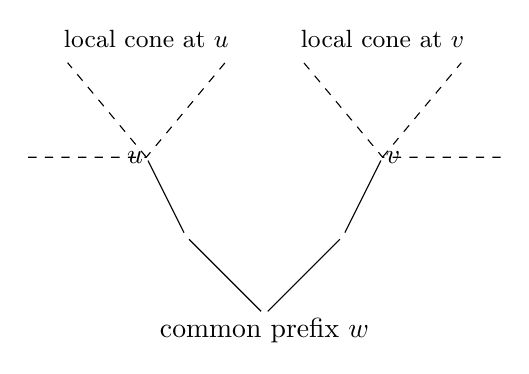
\begin{tikzpicture}[scale=1.0, every node/.style={inner sep=1pt}]
  % Common causal past
  \node (root) at (0,0) {};
  \node (a1) at (-1,1) {};
  \node (b1) at (1,1) {};

  % Two divergent prefixes u and v
  \node (u) at (-1.5,2) {};
  \node (v) at (1.5,2) {};

  % Subcones below u
  \draw[dashed] (-3,2) -- (-1.5,2) -- (-0.5,3.2);
  \draw[dashed] (-1.5,2) -- (-2.5,3.2);

  % Subcones below v
  \draw[dashed] (3,2) -- (1.5,2) -- (0.5,3.2);
  \draw[dashed] (1.5,2) -- (2.5,3.2);

  % Edges in prefix tree
  \draw (root) -- (a1);
  \draw (root) -- (b1);
  \draw (a1) -- (u);
  \draw (b1) -- (v);

  % Labels
  \node[left] at (-1.5,2) {$u$};
  \node[right] at (1.5,2) {$v$};
  \node[below] at (0,0) {common prefix $w$};

  \node at (-1.5,3.5) {\small local cone at $u$};
  \node at (1.5,3.5) {\small local cone at $v$};
\end{tikzpicture}
